% Created 2021-03-19 Fri 21:23
% Intended LaTeX compiler: pdflatex

\documentclass[english]{article}
\usepackage[T1, T2A]{fontenc}
\usepackage[lutf8]{luainputenc}
\usepackage[english, russian]{babel}
\usepackage{minted}
\usepackage{graphicx}
\usepackage{longtable}
\usepackage{hyperref}
\usepackage{xcolor}
\usepackage{natbib}
\usepackage{amssymb}
\usepackage{stmaryrd}
\usepackage{amsmath}
\usepackage{caption}
\usepackage{mathtools}
\usepackage{amsthm}
\usepackage{tikz}
\usepackage{grffile}
\usepackage{extarrows}
\usepackage{wrapfig}
\usepackage{rotating}
\usepackage{placeins}
\usepackage[normalem]{ulem}
\usepackage{amsmath}
\usepackage{textcomp}
\usepackage{capt-of}

\usepackage{geometry}
\geometry{a4paper,left=2.5cm,top=2cm,right=2.5cm,bottom=2cm,marginparsep=7pt, marginparwidth=.6in}

 \usepackage{hyperref}
 \hypersetup{
     colorlinks=true,
     linkcolor=blue,
     filecolor=orange,
     citecolor=black,      
     urlcolor=cyan,
     }

\usetikzlibrary{decorations.markings}
\usetikzlibrary{cd}
\usetikzlibrary{patterns}
\usetikzlibrary{automata, arrows}

\newcommand\addtag{\refstepcounter{equation}\tag{\theequation}}
\newcommand{\eqrefoffset}[1]{\addtocounter{equation}{-#1}(\arabic{equation}\addtocounter{equation}{#1})}


\newcommand{\R}{\mathbb{R}}
\renewcommand{\C}{\mathbb{C}}
\newcommand{\N}{\mathbb{N}}
\newcommand{\rank}{\text{rank}}
\newcommand{\const}{\text{const}}
\newcommand{\grad}{\text{grad}}

\theoremstyle{plain}
\newtheorem{axiom}{Аксиома}
\newtheorem{lemma}{Лемма}
\newtheorem{manuallemmainner}{Лемма}
\newenvironment{manuallemma}[1]{%
  \renewcommand\themanuallemmainner{#1}%
  \manuallemmainner
}{\endmanuallemmainner}

\theoremstyle{remark}
\newtheorem*{remark}{Примечание}
\newtheorem*{solution}{Решение}
\newtheorem{corollary}{Следствие}[theorem]
\newtheorem*{examp}{Пример}
\newtheorem*{observation}{Наблюдение}

\theoremstyle{definition}
\newtheorem{task}{Задача}
\newtheorem{theorem}{Теорема}[section]
\newtheorem*{definition}{Определение}
\newtheorem*{symb}{Обозначение}
\newtheorem{manualtheoreminner}{Теорема}
\newenvironment{manualtheorem}[1]{%
  \renewcommand\themanualtheoreminner{#1}%
  \manualtheoreminner
}{\endmanualtheoreminner}
\captionsetup{justification=centering,margin=2cm}
\newenvironment{colored}[1]{\color{#1}}{}

\tikzset{->-/.style={decoration={
  markings,
  mark=at position .5 with {\arrow{>}}},postaction={decorate}}}
\makeatletter
\newcommand*{\relrelbarsep}{.386ex}
\newcommand*{\relrelbar}{%
  \mathrel{%
    \mathpalette\@relrelbar\relrelbarsep
  }%
}
\newcommand*{\@relrelbar}[2]{%
  \raise#2\hbox to 0pt{$\m@th#1\relbar$\hss}%
  \lower#2\hbox{$\m@th#1\relbar$}%
}
\providecommand*{\rightrightarrowsfill@}{%
  \arrowfill@\relrelbar\relrelbar\rightrightarrows
}
\providecommand*{\leftleftarrowsfill@}{%
  \arrowfill@\leftleftarrows\relrelbar\relrelbar
}
\providecommand*{\xrightrightarrows}[2][]{%
  \ext@arrow 0359\rightrightarrowsfill@{#1}{#2}%
}
\providecommand*{\xleftleftarrows}[2][]{%
  \ext@arrow 3095\leftleftarrowsfill@{#1}{#2}%
}
\makeatother
\author{Ilya Yaroshevskiy}
\date{\today}
\title{Лекция 2}
\hypersetup{
 pdfauthor={Ilya Yaroshevskiy},
 pdftitle={Лекция 2},
 pdfkeywords={},
 pdfsubject={},
 pdfcreator={Emacs 28.0.50 (Org mode )}, 
 pdflang={English}}
\begin{document}

\maketitle
\tableofcontents


\section{Аксиоматическое опредление верояности}
\label{sec:org025b425}
Колмагоров \\

\begin{itemize}
\item \(\Omega\) --- пространство элементарных исходов
\end{itemize}
\begin{deifinition}
Систему \(\mathcal{F} \subset \Omega\) называем \textbf{\(\sigma\)-алгеброй событий} если:
\begin{enumerate}
\item \(\Omega \in \mathcal{F}\)
\item Если \(A \in \mathcal{F}\), то \(\overline{A} \in \mathcal{F}\)
\item Если \(A_1, A_2, \dots \in \mathcal{F}\), то \(\bigcup_{i=1}^{+ \infty} A_i \in \mathcal{F}\)
\end{enumerate}
\end{deifinition}
\begin{remark}
Свойства:
\begin{enumerate}
\item \(\emptyset \in \mathcal{F}\), т.к. \(\overline{\Omega} = \emptyset \in \mathcal{F}\)
\item Если \(A_1, A_2, \dots \in \mathcal{F}\), то \(\bigcap_{i = 1}^{+ \infty} A_i \in \mathcal{F}\)
\begin{proof}
\-\\
\(A_1, A_2, \dots \in \mathcal{F} \Rightarrow \overline{A_1}, \overline{A_2}, \dots \in \mathcal{F} \Rightarrow \bigcup_{i = 1}^{+ \infty} \overline{A_i} \in \mathcal{F} \Rightarrow \overline{\bigcup_{i = 1}^{+ \infty}\overline{A_i}} = \bigcap_{i = 1}^{+ \infty} A_i \in \mathcal{F}\)
\end{proof}
\item \begin{enumerate}
\item \(F = \{\Omega, \emptyset\}\)
\item \(F = \{\Omega, \emptyset, A, \overline{A}\}\)
\end{enumerate}
\end{enumerate}
\end{remark}
\begin{definition}
\(] \Omega\) --- пространство элементарных исходовб \(\mathcal{F}\) -- его \(\sigma\)-алгебра.
\textbf{Вероятностью} на \((\Omega, \mathcal{F})\) обозначается функция \(P(A): \mathcal{F} \to \R\) со свойствами:
\begin{enumerate}
\item \(P(A) \ge 0\) --- свойство \textbf{неотрицательности}
\item Если события \(A_1, A_2, \dots\) --- попарно несовместны(\(\forall i,j:\ A_i \cap A_j = \emptyset\)),
то: \[ P(\bigsqcup_{i = 1}^{+ \infty} A_i) = \sum_{i = 1}^{+ \infty} P(A_i) \] --- свойство \textbf{счетной аддитивности}
\item \(P(\Omega) = 1\) --- свойство \textbf{нормированности}
\end{enumerate}
\end{definition}

\begin{definition}
Тройка \((\Omega, \mathcal{F}, P)\) --- \textbf{вероятностное пространство}
\end{definition}
\begin{remark}
Свойства:
\begin{enumerate}
\item \(P(\emptyset) = 0\)
\begin{proof}
\(\emptyset\) и \(\Omega\) --- несовместные события
\[ P(\underbrace{\emptyset + \Omega}_\Omega) = P(\emptyset) + P(\Omega) = 1 \]
\[ P(\emptyset) + 1 = 1 \]
\[ P(\emptyset) = 0 \]
\end{proof}
\item Формула обратной вероятнсоти \[ P(A) = 1 - P(\overline{A}) \]
\begin{proof}
\(A\) и \(\overline{A}\) --- несовместные, \(A \cup \overline{A} = \Omega\)
\[ P(A + \overline{A}) = P(A) + P(\overline{A}) = 1 \Rightarrow P(A) = 1 - P(\overline{A}) \]
\end{proof}
\item \(0 \le P(A) \le 1\)
\begin{proof}
\-
\begin{enumerate}
\item \(P(A) \ge 0\)
\item \(P(A) = 1 - P(\overline{A}) \le 1\)
\end{enumerate}
\end{proof}
\end{enumerate}
\end{remark}
\begin{axiom}
Пусть имеется убывающая цепочка событий \(A_1 \supset A_2 \supset A_3 \supset \dots\), \(\bigcap_{i = 1}^{+ \infty} A_i = \emptyset\) \\
\uline{Тогда} \(P(A_n) \xrightarrow[n \to \infty]{} 0\)
\end{axiom}
\begin{remark}
При непрерывном изменении области \(A\subset \R^n\) соответствующая вероятность также должна изменяться непрерывно.
Аксиома непрерывности следует из аксиомы счетной аддитивности
\end{remark}
\begin{proof}
\-
\begin{center}
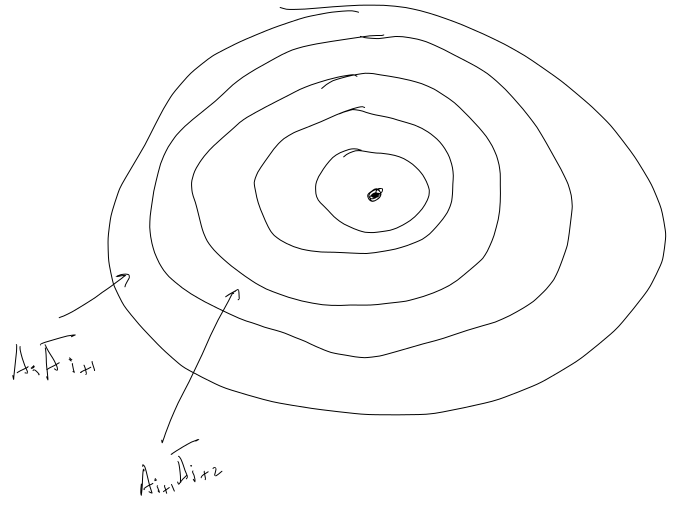
\includegraphics[scale=0.3]{2_1.png}
\end{center}
\[ A_n = \sum_{i = n}^{+ \infty} A_i\overline{A_{i + 1}} \cup \bigcap_{i = n}^{+ \infty}A_i \]
т.к. эти события несовместны
\[ P(A_n) = \sum_{i = n}^{+ \infty}P(A_i\overline{A_{i + 1}}) + P(\bigcap_{i = n}^{+\infty} A_i) \]
т.к. \(P(\bigcap_{i = 1}^{ + \infty} A_i) = \emptyset\) и \(\bigcap_{i = n}^{ +\infty}A_i = \bigcap_{i = 1}^{ + \infty}A_i\), то \(P(\bigcap_{i = n}^{ + \infty} A_i) = 0\) \\
\[ P(A_n) = \sum_{i = n}^{ + \infty} P(A_i \overline{A_{i + 1}}) \]
\[ \sum_{i = 1}^{ + \infty}P(A_i\overline{A_{i + 1}}) = P(A_i) \]
\[ P(A_n) \xrightarrow[n \to + \infty]{} 0 \]
\end{proof}
\begin{remark}
Аксимома счетной аддитивности следует из аксиомы непрерывности и свойства конечной аддитивности
\end{remark}
\subsection{Свойства операция сложения, умножения}
\label{sec:org849d210}
\begin{definition}
\-
\begin{enumerate}
\item Свойство дистрибутивности \(A\cdot (B + C) = AB + AC\)
\item Формула сложения. Если \(A\) и \(B\) --- несовместны, то \(P(A + B) = P(A) + P(B)\) \\
если совместны, то \(P(A + B) = P(A) + P(B) - P(AB)\)
\begin{proof}
\-
\begin{center}
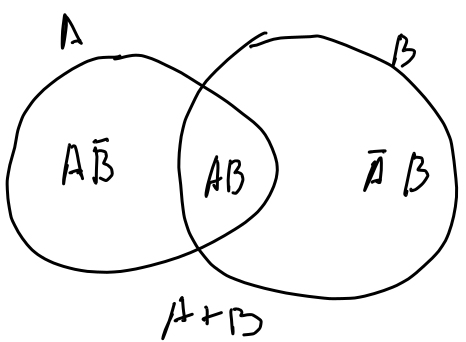
\includegraphics[scale=0.4]{2_2.png}
\end{center}
\[ A + B = A\overline{B} + AB + \overline{A}B \Rightarrow P(A + B) = P(A\overline{B}) + P(AB) + P(\overline{A}B) = \]
\[ = P(A\overline{B}) + P(AB) + (P(\overline{A}B) + P(AB)) - P(AB) = P(A) + P(B) - P(AB) \]
\end{proof}
\end{enumerate}
\end{definition}
\begin{task}
\(n\) писем раскладываются в \(n\) конвертов. Найти вероятнсоть того что
хотя бы одно письмо попадет в свой коверт. Чему равна эта вероятность
при \(n \to + \infty\)
\end{task}
\begin{solution}
\(A_i\) --- \(i\) письмо попало в свой коверт \\
\(A\) --- хотя бы одно письмо попало в свой конверт
\[ A = A_1 + A_2 + \dots + A_n \]
\[ P(A_i) = \frac{1}{n},\ P(A_iA_j) = \frac{1}{A^2_n},\ P(A_iA_jA_k) = \frac{1}{A^3_n}, \dots P(A_1A_2\dots A_n) = \frac{1}{n!}\]
\[ P(A) = n\cdot\frac{1}{n} - C^2_n\cdot\frac{1}{A^2_n} + \dots + (-1)^{n + 1}\frac{1}{n!} = 1 - \frac{1}{2!} + \frac{1}{3!} - \dots + (-1)^{n + 1}\frac{1}{n!} \]
\[ e^{-1} = 1 - 1 + \frac{1}{2!} - \frac{1}{3!} + \dots \]
\[ P(A) \xrightarrow[n \to +\infty]{} 1 - e^{-1} \]
\end{solution}
\subsection{Независимые события}
\label{sec:org54b7dc7}
\begin{remark}
\(\Omega = n\), \(|A| = m_1\), \(|B| = m_2\) \\
\(|\Omega \times \Omega| = n^2\), \(AB = m_1m_2\)
\end{remark}
\begin{definition}
События \(A\) и \(B\) называются \textbf{независимыми}, если \(P(AB) = P(A)P(B)\)
\end{definition}
\begin{remark}
Свойство: если \(A\) и \(B\) --- независимы, то \(A\) и \(\overline{B}\) --- независимы
\end{remark}
\begin{proof}
\(P(A) = P(A(B + \overline{B})) = P(AB + A\overline{B}) = P(AB) + P(A\overline{B}) \Rightarrow P(A\overline{B}) = P(A) - P(AB) = P(A) - P(A)\cdot P(B) = P(A)\cdot(1 - P(B)) = P(A)\cdot P(\overline{B})\) \(\Rightarrow\) \(A\) и \(\overline{B}\) --- независимы
\end{proof}
\begin{definition}
События \(A_1,A_2, \dots, A_n\) называются \textbf{независимыми в совокупности}, если для любого набора \(1 \le i_1, i_2, \dots, i_k \le n\ P(A_{i_1}A_{i_2}\dots A_{i_k}) = P(A_{i_1})P(A_{i_2})\dots P(A_{i_k})\)
\end{definition}
\begin{remark}
Если события независимы в совокупности, то события независимы попарно(при \(k = 2\)). Обратное неверно
\end{remark}
\begin{examp}[Берштейна]
Три грани правильного тетраэдра выкрашены в красный, синий, зленый цвета, а четвертая грань во все эти три цвета \\
\(] A\) --- грань содержит красный цвет, \(B\) --- синий, \(C\) --- зеленый \\
\[ P(A) = P(B) = P(C) = \frac{2}{4} = \frac{1}{2} \]
\[ P(AB) = P(AC) = P(BC) = \frac{1}{4} \]
\[ P(AB) = \frac{1}{4} = \frac{1}{2}\cdot\frac{1}{2} = P(A)P(B) \] \(\Rightarrow\) все события попарно независимы
\[ P(ABC) = \frac{1}{4} \neq P(A)P(B)P(C) = \frac{1}{8} \] \(\Rightarrow\) события не независимы в совокупности
\end{examp}
\begin{remark}
Если в условии есть ``хотябы``, т.е. требуется найти вероятность совместных независимых событий, то применяем формулу обратной вероятности
\end{remark}
\begin{task}
Найти веротяность того, что при 4 бросаниях кости, хотябы один раз выпадет шестерка.
\end{task}
\begin{solution}
\(] A_1\) --- при 1 броске "6", \(A_2\) --- при 2х бросках "6", \dots{}, \(A\) --- хотя бы один раз "6"
\[ A = A_1 + A_2 + A_3 + A_4 \]
\[ P(A_1) = P(A_2) = P(A_3) = P(A_4) = \frac{1}{6} \]
\[ P(\overline{A_1}) = P(\overline{A_2}) = P(\overline{A_3}) = P(\overline{A_4}) = \frac{5}{6} \]
\(\overline{A}\) --- ни разу не выпадет
\[ \overline{A} = \overline{A_1}\cdot\overline{A_2}\cdot\overline{A_3}\cdot\overline{A_4} \]
\[ P(\overline{A}) = \left(\frac{5}{6}\right)^4  \]
\[ P(A) = 1 - P(\overline{A}) \]
\end{solution}
\begin{task}
Два стрелка стреляют по мишени. Вероятность попадания первого --- \(0.6\), второго --- \(0.8\)
\end{task}
\begin{solution}
\(A_1\) --- 1й попал \\
\(A_2\) --- 2й попал \\
\(A\) --- один попал
\[ A = A_1\cdot\overline{A_2} + \overline{A_1}A_2 \]
\[ P(A)  = P(A)\cdot P(\overline{A_2}) + P(\overline{A_1})\cdot P(A_2) \]
\end{solution}
\end{document}
